\section{Функциональные последовательности и ряды}

\begin{definition}
	Пусть $\{f_n\}_{n = 0}^\infty$ "--- последовательность функций, определенных на области $G \subset \Cm$, функция $f$ определена на $G$. Последовательность $\{f_n\}$ \textit{сходится локально равномерно} к $f$ на области $G$, если $\forall z_0 \in G: \exists \epsilon > 0: f_n \convu_{B_\epsilon(z_0)} f$. Обозначение "--- $f_n \convlr f$.
\end{definition}

\begin{proposition}
	Пусть выполнены следующие условия:
	\begin{enumerate}
		\item Функции $f_0, f_1, \dotsc$ непрерывны на области $G \subset \Cm$
		\item $f_n \convlr f$ на $G$
	\end{enumerate}
	
	Тогда $f$ непрерывна на $G$.
\end{proposition}

\begin{proof}
	Аналогично вещественному случаю.
\end{proof}

\begin{definition}
	Пусть $\{f_n\}_{n = 0}^\infty$ "--- последовательность функций, определенных на области $G \subset \Cm$. Ряд $\sum_{k = 0}^\infty f_k$ \textit{сходится локально равномерно} на $G$, если последовательность его \textit{частных сумм} $S_n := \sum_{k = 0}^nf_k$ локально равномерно сходится к некоторой определенной на $G$ функции $S$, называемой \textit{суммой} ряда.
\end{definition}

\begin{proposition}
	Пусть выполнены следующие условия:
	\begin{enumerate}
		\item Функции $f_0, f_1, \dotsc$ непрерывны на области $G \subset \Cm$
		\item Ряд $\sum_{k = 0}^\infty f_k$ локально равномерно сходится к сумме $S$ на $G$
	\end{enumerate}
	
	Тогда $S$ непрерывна на $G$.
\end{proposition}

\begin{proof}
	Воспользуемся утверждением о функциональных последовательностях для последовательности $\{S_n\}_{n=0}^\infty$.
\end{proof}

\begin{proposition}
	Пусть $\{f_n\}_{n = 0}^\infty$ "--- последовательность функций, определенных на области $G \subset \Cm$, функция $f$ определена на $G$. Тогда $f_n \convlr f$ на $G$ $\lra$ для любого компакта $K \subset G$ выполнено $f_n \convu_K f$.
\end{proposition}

\begin{proof}~
	\begin{itemize}
		\item[$\ra$]Для произвольной точки $z \in K$ выберем окрестность $B(z)$ такую, что $f_n \convu_{B(z)} f$. Тогда $K \subset \bigcup_{z \in K}B(z)$, и, в силу компактности, можно выбрать конечный набор $z_1, \dotsc, z_m$ такой, что $K \subset \bigcup_{k=1}^mB(z_k)$. Поскольку для любого $k \in \{1, \dotsc, m\}$ выполнено $f_n \convu_{B_k(z)} f$, то $f_n \convu_K f$.
		
		\item[$\la$]Зафиксируем произвольную точку $z_0 \in G$ и выберем $\delta > 0$ такое, что $\overline{B_\delta(z_0)} \subset G$, тогда $f_n \convu_{\overline{B_\delta(z_0)}} f$.\qedhere
	\end{itemize}
\end{proof}

\begin{proposition}
	Пусть выполнены следующие условия:
	\begin{enumerate}
		\item Функции $f_0, f_1, \dotsc$ непрерывны на области $G \subset \Cm$
		\item $f_n \convlr f$ на $G$
		\item $\gamma$ "--- кусочно-гладкая кривая такая, что $M(\gamma) \subset G$
	\end{enumerate}
	
	Тогда верно следующее равенство:
	\[\int_\gamma f_ndz \xrightarrow{n \to \infty} \int_\gamma fdz\]
\end{proposition}

\begin{proof}
	Из условия следует, что $f$ непрерывна на $G$, а $M(\gamma)$ "--- компакт, поскольку $M(\gamma)$ является непрерывным образом отрезка. Тогда $f_n \convu_{M(\gamma)} f$, и выполнено следующее:
	\[\left|\int_\gamma f_ndz - \int_\gamma fdz\right| = \left|\int_\gamma (f_n - f)dz\right| \le \left(\max_{z \in M(\gamma)}|f_n(z) - f(z)|\right)|\gamma| \xrightarrow{n \to \infty} 0\]
	
	Получено требуемое.
\end{proof}

\begin{note}
	Переформулируем утверждение выше для случая функциональных рядов. Пусть выполнены следующие условия:
	\begin{enumerate}
		\item Функции $f_0, f_1, \dotsc$ непрерывны на области $G \subset \Cm$
		\item Ряд $\sum_{n=0}^\infty f_n$ сходится локально равномерно на $G$
		\item $\gamma$ "--- кусочно-гладкая кривая такая, что $M(\gamma) \subset G$
	\end{enumerate}
	
	Тогда верно следующее равенство:
	\[\int_\gamma \left(\sum_{n=0}^\infty f_n\right)dz = \sum_{n=0}^\infty \left(\int_\gamma f_ndz\right)\]
\end{note}

\begin{definition}
	Пусть $\{f_n\}_{n = 0}^\infty$ "--- последовательность функций, определенных на множестве $E \subset \Cm$. Ряд $\sum_{n=0}^\infty f_n$ \textit{сходится регулярно} на $E$, если ряд $\sum_{n=0}^\infty |f_n|$ сходится равномерно на $E$.
\end{definition}

\begin{note}
	Из регулярной сходимости следует равномерная сходимость в силу критерия Коши и неравенства треугольника.
\end{note}

\begin{theorem}[признак Вейерштрасса]
	Пусть выполнены следующие условия:
	\begin{enumerate}
		\item Функции $f_0, f_1, \dotsc$ определены на множестве $E \subset \Cm$
		\item $\forall n \in \mathbb{N} \cup \{0\} : \exists a_n > 0: \forall z \in E: |f_n(z)| \le a_n$
		\item Ряд $\sum_{n=0}^\infty a_n$ сходится
	\end{enumerate}
	
	Тогда ряд $\sum_{n=0}^\infty f_n$ сходится регулярно на $E$.
\end{theorem}

\begin{proof}
	Аналогично вещественному случаю.
\end{proof}

\section{Cтепенные ряды}

\begin{definition}
	Пусть $z_0 \in \Cm$ и $c_0, c_1, \dotsc \in \Cm$. \textit{Степенным рядом} называется выражение вида $\sum_{n=0}^\infty c_n(z - z_0)^n$. Точка $z_0$ называется \textit{центром разложения}.
\end{definition}

\begin{note}
	Для удобства обозначений, в дальнейшем мы будем рассматривать только степенные ряды с центром в нуле, то есть выражения вида $\sum_{n=0}^\infty c_nz^n$. Любой степенной ряд можно привести к такому виду заменой координат.
\end{note}

\pagebreak

\begin{definition}
	\textit{Радиусом сходимости} степенного ряда $\sum_{n=0}^\infty c_nz^n$ называется величина $R := \sup\{|z| : \text{ряд }\sum_{n=0}^\infty c_nz^n\text{ сходится}\}$. \textit{Кругом сходимости} ряда называется множество $K := \{z \in \Cm : |z| < R\}$.
\end{definition}

\begin{theorem}[Абеля]
	Пусть степенной ряд $\sum_{n=0}^\infty c_nz^n$ имеет радиус сходимости $R > 0$ и круг сходимости $K$. Тогда:
	\begin{enumerate}
		\item Ряд $\sum_{n=0}^\infty c_nz^n$ сходится абсолютно для любого $z \in K$
		\item Ряд $\sum_{n=0}^\infty c_nz^n$ сходится регулярно в круге $K_r := \{z \in \Cm: |z| \le r\}$ при любом $r < R$
	\end{enumerate}
\end{theorem}

\begin{proof}
	Достаточно доказать вторую часть. Зафиксируем $r < R$, тогда, по определению, $\exists z_1 \in \Cm$ такое, что $|z_1| > r$ и ряд $\sum_{n=0}^\infty c_nz_1^n$ сходится. Следовательно, $c_nz_1^n \xrightarrow{n \to \infty} 0$, тогда существует $M > 0$ такое, что для любого $n \in \N \cup \{0\}$ выполнено $|c_nz_1^n| \le M$. Тогда для любого $n \in \N \cup \{0\}$ и любого $z \in K_r$ имеем:
	\[\left|c_nz^n\right| = \left|c_nz_1^n\right|\left|\frac{z}{z_1}\right|^n \le M\left(\frac{r}{|z_1|}\right)^n\]
	
	По признаку Вейерштрасса, получено требуемое.
\end{proof}

\begin{note}
	Если радиус сходимости $R$ ряда $\sum_{n=0}^\infty c_nz^n$ конечен, то при $z \in \Cm$ таких, что $|z| > R$, ряд расходится по определению радиуса сходимости. Поведение ряда на границе круга сходимости может быть разным.
\end{note}

\begin{proposition}
	Пусть степенной ряд $\sum_{n=0}^\infty c_nz^n$ имеет радиус сходимости $R > 0$ и круг сходимости $K$. Тогда:
	\begin{enumerate}
		\item Ряд $\sum_{n = 1}^\infty nc_nz^{n-1}$ сходится абсолютно для любого $z \in K$
		\item Ряд $\sum_{n = 1}^\infty nc_nz^{n-1}$ сходится регулярно в круге $K_r$ при любом $r < R$
	\end{enumerate}
\end{proposition}

\begin{proof}
	Снова достаточно доказать вторую часть. Зафиксируем $r < R$ и число $z_1 \in K$ такое, что $|z_1| > r$. Аналогично теореме выше, выберем $M > 0$ такое, что для любого $n \in \N \cup \{0\}$ выполнено $|c_nz_1^n| \le M$. Тогда для любого $z \in K_r$ имеем:
	\[\left|nc_nz^{n-1}\right| = \left|nc_nz_1^{n-1}\right|\left|\frac{z}{z_1}\right|^{n-1} \le \frac{nM}{|z_1|}\left(\frac{r}{|z_1|}\right)^{n-1}\]
	
	По признаку Вейерштрасса, получено требуемое.
\end{proof}

\begin{corollary}
	Ряды $\sum_{n=0}^\infty c_nz^n$ и $\sum_{n = 1}^\infty nc_nz^{n-1}$ сходятся локально равномерно на круге сходимости $K$ первого ряда.
\end{corollary}

\begin{proof}
	Для произвольной точки $z \in K$ можно выбрать такой круг $K_r \supset B(z)$, на котором ряды сходятся регулярно.
\end{proof}

\begin{corollary}
	Функции $f(z) := \sum_{n = 0}^\infty c_nz^n$, $g(z) := \sum_{n = 0}^\infty nc_nz^{n-1}$ непрерывны на круге сходимости $K$ первого ряда.
\end{corollary}

\begin{corollary}
	Пусть степенной ряд $\sum_{n=0}^\infty c_nz^n$ имеет радиус сходимости $R > 0$. Тогда и ряд $\sum_{n = 1}^\infty nc_nz^{n-1}$ имеет радиус сходимости $R$.
\end{corollary}

\begin{proof}
	Пусть $\sum_{n = 1}^\infty nc_nz^{n-1}$ имеет радиус сходимости $R_1$. Тогда, по доказанному выше, $R_1 \ge R$. C другой стороны, если при некотором $z \in \Cm$ ряд $\sum_{n = 1}^\infty nc_nz^{n-1}$ сходится, то сходится и ряд $\sum_{n = 1}^\infty nc_nz^n$, и ряд $\sum_{n = 0}^\infty c_nz^n$. Значит, $R_1 \le R$.
\end{proof}

\begin{corollary}
	Пусть степенной ряд $\sum_{n=0}^\infty c_nz^n$ имеет радиус сходимости $R > 0$ и круг сходимости $K$. Тогда функция $g(z) := \sum_{n = 1}^\infty nc_nz^{n-1}$ имеет первообразную на $K$.
\end{corollary}

\begin{proof}
	Пусть $\gamma$ "--- замкнутая кусочно-гладкая кривая такая, что $M(\gamma) \subset K$. Поскольку ряд $\sum_{n = 1}^\infty c_nnz^{n-1}$ сходится равномерно на $M(\gamma)$, то, интегрируя почленно, имеем:
	\[\int_\gamma gdz = \sum_{n = 1}^\infty \int_\gamma nc_nz^{n-1}dz = 0\]
	
	Значит, в силу произвольности выбора кривой $\gamma$, $g$ имеет первообразную на $K$.
\end{proof}

\begin{note}
	В частности, одной из первообразных функции $g(z)$ является следующая функция:
	\[h(z) := \int_0^zgdw = \sum_{n=1}^\infty \int_0^znc_nw^{n-1}dw = \sum_{n=1}^\infty c_nz^n\]
	
	Почленное интегрирование возможно, поскольку ряд $\sum_{n = 1}^\infty n c_nw^{n-1}$ сходится равномерно на любом отрезке вида $[0, z] \subset K$.
\end{note}

\begin{proposition}
	Пусть степенной ряд $\sum_{n=0}^\infty c_nz^n$ имеет радиус сходимости $R > 0$ и круг сходимости $K$. Тогда функция $f(z) := \sum_{n = 0}^\infty c_nz^{n}$ регулярна на $K$, причем для любого $z \in K$ выполнено $f'(z) = \sum_{n=1}^\infty nc_nz^{n-1}$ на $K$.
\end{proposition}

\begin{proof}
	Функция $g(z) := \sum_{n = 1}^\infty nc_nz^{n-1}$ имеет первообразную $h(z) = \sum_{n=1}^\infty c_nz^n \hm= f(z) - c_0$ на $K$, поэтому $f$ "--- тоже первообразная функции $g$ на $K$. Кроме того, $g$ непрерывна на $K$ в силу равномерной сходимости ряда $nc_nz^{n-1}$.
\end{proof}

\begin{corollary}
	Пусть степенной ряд $\sum_{n=0}^\infty c_nz^n$ имеет радиус сходимости $R > 0$ и круг сходимости $K$. Тогда функция $f(z) := \sum_{n = 0}^\infty c_nz^{n}$ бесконечно дифференцируема на $K$.
\end{corollary}

\begin{proof}
	Последовательно применим утверждение выше к рядам, получаемым из $\sum_{n=0}^\infty c_nz^n$ многократным почленным дифференцированием.
\end{proof}

\begin{note}
	В частности, $f^{(n)}(0) =c_nn!$ для любого $n \in \N$. Тогда:
	\[f(z) = \sum_{n=0}^\infty \frac{f^{(n)}(0)}{n!}z^n,~|z| < R\]
	
	Значит, степенной ряд $\sum_{n=0}^\infty c_nz^n$ является рядом Тейлора своей суммы. В случае произвольного центра $z_0 \in \Cm$ у степенного ряда, равенство выше принимает следующий вид:
	\[f(z) = \sum_{n=0}^\infty \frac{f^{(n)}(z_0)}{n!}(z - z_0)^n,~|z - z_0| < R\]
\end{note}

\begin{note}
	Пусть функция $f$ может быть представлена в виде степенного ряда в круге $\{z \in \Cm : |z - z_0| < R\}$, где $z_0 \in \Cm$, $R > 0$. Тогда это представление единственно, поскольку оно совпадает с рядом Тейлора функции $f$.
\end{note}

\section{Интеграл Коши и бесконечная дифференцируемость}

\begin{definition}
	Пусть $\gamma$ "--- кусочно-гладкая кривая, $z = \sigma(t)$, $t \in [a, b]$, "--- ее параметризация, и функция $f$ такова, что композиция $f\circ\sigma$ непрерывна на $[a, b]$. \textit{Интегралом Коши} называется функция, определенная вне множества $M(\gamma)$, следующего вида:
	\[F(z) := \frac1{2\pi i}\int_\gamma \frac{f(w)}{w - z}dw\]
\end{definition}

\begin{theorem}
	Пусть $F$ "--- интеграл Коши для кривой $\gamma$ и функции $f$, числа $z_0 \in \Cm$, $R > 0$ таковы, что круг $K := \{z \in \Cm: |z - z_0| < R\}$ не пересекается с $M(\gamma)$. Тогда на $K$ интеграл Коши $F$ может быть представлен степенным рядом с центром $z_0$.
\end{theorem}

\begin{proof}
	По условию, $R \le d := \inf\{|z_0 - w| : w \in M(\gamma)\}$. Зафиксируем $z \in K$, тогда $|z - z_0| < R \le d$, и для любого $w \in M(\gamma)$ имеем:
	\[\frac1{w - z} = \frac1{(w-z_0) - (z - z_0)} = \frac1{w-z_0}\cdot \frac1{1 - \frac{z-z_0}{w - z_0}} = \sum_{n=0}^\infty\frac{(z-z_0)^n}{(w-z_0)^{n + 1}}\]
	
	При любом $w \in M(\gamma)$ выполнено следующее неравенство:
	\[\left|\frac{(z-z_0)^n}{(w-z_0)^{n + 1}}\right| \le \frac{1}{|z - z_0|}\left(\frac{|z - z_0|}{d}\right)^{n+1}\]
	
	Тогда, по признаку Вейерштрасса, ряд, представляющий функцию $\frac1{w - z}$, сходится равномерно на $M(\gamma)$, тогда на $M(\gamma)$ равномерно сходится и ряд следующего вида:
	\[\frac1{2\pi i} \cdot\frac{f(w)}{w-z} = \sum_{n=0}^\infty\frac1{2\pi i}\cdot \frac{f(w)}{(w-z_0)^{n + 1}}(z-z_0)^n\]
	
	Интегрируя обе части равенства выше, получим требуемое:
	\[F(z) = \frac1{2\pi i} \int_\gamma \frac{f(w)}{w-z}dw = \sum_{n=0}^\infty\left(\frac1{2\pi i} \int_\gamma\frac{f(w)}{(w-z_0)^{n + 1}}dw\right)(z-z_0)^n \qedhere\]
\end{proof}

\begin{corollary}
	Интеграл Коши $F(z)$ бесконечно дифференцируем на $\Cm \bs M(\gamma)$, причем для любых $z \in \Cm$ и $n \in \N$ выполнено равенство:
	\[F^{(n)}(z) = \frac{n!}{2\pi i} \int_\gamma\frac{f(w)}{(w-z)^{n + 1}}dw\]
\end{corollary}

\begin{definition}
	Множество функций, бесконечно дифференцируемых на области $G \subset \Cm$, обозначается через $C^\infty(G)$.
\end{definition}

\begin{theorem}
	Пусть $z_0 \in \Cm$, $R > 0$, функция $f$ регулярна на $K := \{z \in \Cm : |z - z_0| < R\}$. Тогда $f \in C^\infty(K)$, и $f$ представима рядом Тейлора в любой точке $z \in K$:
	\[f(z) = \sum_{n = 0}^\infty \frac{f^{(n)}(z_0)}{n!}(z - z_0)^n\]
\end{theorem}

\begin{proof}
	Зафиксируем $R_1 < R$ и положим $K_1 := \{z \in \Cm: |z - z_0| < R_1\}$. Тогда $f \in C^1(\overline{K_1})$, и по интегральной формуле Коши для любого $z \in K_1$ выполнено следующее:
	\[f(z) = \frac{1}{2\pi i}\int_{\partial K_1}\frac{f(w)}{w - z}dw\]
	
	Значит, $f$ является интегралом Коши на $K_1$, поэтому на $K_1$ функция $f$ бесконечно дифференцируема и представима рядом Тейлора. В силу произвольности выбора $R_1$, получено требуемое.
\end{proof}

\begin{note}
	Анализируя доказательство теоремы выше, получим следующее равенство для любых чисел $z \in K_1$ и $n \in \N$:
	\[f^{(n)}(z) = \frac{n!}{2\pi i}\int_{\partial K_1}\frac{f(w)}{(w - z)^{n+1}}dw\]
	
	Это равенство называется \textit{интегральной формулой Коши для производной порядка $n$}.
\end{note}

\begin{theorem}[Мореры]
	Пусть функция $f$ непрерывна на области $G \subset \Cm$ и для любой замкнутой кусочно-гладкой кривой $\gamma$ такой, что $M(\gamma) \subset G$, выполнено равенство:
	\[\int_\gamma fdz = 0\]
	
	Тогда $f$ регулярна на $G$.
\end{theorem}

\begin{proof}
	По условию, функция $f$ имеет первообразную на $G$, причем ее первообразная $F$ регулярна на $G$ в силу непрерывности функции $f$. К каждой точке из $G$ применима предыдущая теорема, откуда $F \in C^\infty(G)$. Но тогда и $f = F' \in C^\infty(G)$.
\end{proof}

\begin{example}
	Пусть $K_1 = \{z \in \Cm: |z| < 1\}$, тогда граница круга $\partial K_1$ задает кривую $\gamma$ с параметризацией $w = e^{it}$, $t \in [-\pi, \pi]$. Тогда для функции $f(z) = e^z$ и любого $n \in \N$ выполнено следующее равенство:
	\[1 = f^{(n)}(0) = \frac{n!}{2\pi i} \int_\gamma \frac{e^w}{w^{n+1}}dw = \frac{n!}{2\pi i} \int_{-\pi}^\pi \frac{e^{e^{it}}\cdot ie^{it}}{e^{it(n+1)}}dt = \frac{n!}{2\pi} \int_{-\pi}^\pi e^{\cos{t} + i(\sin{t} - tn)}dt\]
	
	Отсюда получаем следующее:
	\[\int_{0}^\pi e^{\cos{t}}\cos{(\sin{t} - tn)}dt = \frac\pi{n!}\]
\end{example}

\begin{note}
	Поскольку любую область $G \subset \Cm$ можно представить в виде объединения кругов, то для любой функции $f \in C^1(G)$ выполнено, что $f \in C^\infty(G)$.
\end{note}

\section{Гармонические функции}

\begin{definition}
	Пусть $G \subset \R^2$ "--- область. Функция $u : \R^2 \to \R$ называется \textit{гармонической} на $G$, если выполнены следующие условия:
	\begin{enumerate}
		\item $u \in C^2(G)$
		\item $u''_{xx} + u''_{yy} \equiv 0$ на $G$
	\end{enumerate}
\end{definition}

\begin{proposition}
	Пусть функция $f(z) = f(x + iy) = u(x, y) + iv(x, y)$ регулярна на области $G \subset \Cm$. Тогда функции $u, v$ "--- гармонические на $G$.
\end{proposition}

\begin{proof}
	Поскольку $f \in C^\infty(G)$, то и $u, v \in C^\infty(G)$. По условиям Коши-Римана, на $G$ выполнено $u'_x \equiv v'_y$ и $u'_y \equiv -v'_x$. Дифференцируя тождества по $x$ и $y$ соответственно и складывая их, получим:
	\[u''_{xx} + u''_{yy} \equiv v''_{yx} - v''_{xy} \equiv 0\]
	
	Аналогично, $v''_{xx} + v''_{yy} \equiv 0$ на $G$.
\end{proof}

\begin{proposition}
	Пусть выполнены следующие условия:
	\begin{enumerate}
		\item $G \subset \R^2$ "--- односвязная область
		\item Функция $u$ "--- гармоническая на $G \subset \R^2$
	\end{enumerate}
	
	Тогда существует гармоническая на $G$ функция $v$ такая, что на $G$ регулярна функция $f(z) = f(x + iy) := u(x, y) + iv(x, y)$.
\end{proposition}

\begin{proof}
	Поскольку $u$ "--- гармоническая, то на $G$ выполнено $u_{xx}'' + u_{yy}'' \equiv 0$, тогда интеграл ниже не зависит от выбора кусочно-гладкой кривой, соединяющей фиксированные точки $(x_0, y_0), (x, y) \in G$:
	\[v(x, y) := \int_{(x_0, y_0)}^{(x, y)}-u'_ydx + u'_xdy\]
	
	Значит, $v(x, y)$ "--- потенциальная функция поля $(-u'_y, u'_x)$, поэтому на $G$ выполнены тождества $v'_x \equiv -u'_y$ и $v'_y \equiv u'_x$. Тогда $v$ "--- гармоническая на $G$, и $f \in C^1(G)$.
\end{proof}

\begin{note}
	Функция $v$ в теореме выше восстанавливается однозначно с точностью до константы как решение системы дифференциальных уравнений, задаваемой условиями Коши-Римана. Аналогично доказывается, что по гармонической функции $v$ однозначно с точностью до константы восстанавливается функция $u$. Требование односвязности при этом существенно, что показывает пример ниже.
\end{note}

\begin{example}
	Пусть $G := \{z \in \Cm : \frac12 < |z| < 2\}$, $u(x, y) := \ln(x^2 + y^2)$. Можно проверить, что функция $u$ "--- гармоническая на $G$, однако не существует гармонической на $G$ функции $v$ такой, что $f(z) = f(x + iy) = u(x, y) + iv(x, y)$ регулярна на $G$. Предположим, что такая функция $v$ существует, тогда:
	\[f'(x) = u'_x + iv'_x = u'_x - iu'_y = \frac{2}{x + iy} = \frac 2z\]
	
	Значит, функция $f$ является первообразной для функции $\frac 2z$ на $G$. При этом для круга $K := \{z \in \Cm: |z| = 1\}$ выполнено следующее равенство:
	\[\int_{K} \frac 2zdz = 4\pi i \ne 0\]
	
	Значит, функция $\frac2z$ не может иметь первообразной на $G$ --- противоречие.
\end{example}

\section{Теорема единственности}

\begin{definition}
	Точка $z_0 \in \Cm$ называется \textit{нулем} функции $f$, если $f(z_0) = 0$.
\end{definition}

\begin{note}
	Пусть $z_0 \in \Cm$, $R > 0$. Мы уже знаем, что если функция $f$ регулярна на круге $K := \{z \in \Cm: |z - z_0| < R\}$, то существует единственное разложение функции $f$ в ряд:
	\[f(z) = \sum_{n=0}^\infty c_n(z - z_0)^n\]
	
	Если $f(z_0) = 0$, то и $c_0 = 0$. Возможны два случая:
	\begin{enumerate}
		\item Если $\forall n \in \N\cup \{0\}: c_n = 0$, то $f \equiv 0$ на $K$
		\item Если для некоторого $m \in \N$ выполнено, что $\forall n \in \{0, \dotsc, m - 1\}: c_n = 0$, но $c_m \ne 0$, то функция $f$ имеет следующий вид:
		\[f(z) = (z - z_0)^m\left(\sum_{n = 0}^\infty c_{n + m}(z - z_0)^n\right)\]
		
		Ряд $\sum_{n = 0}^\infty c_{n + m}(z - z_0)^n$ сходится на круге $K$, как исходный ряд, поэтому задаваемая им функция $h(z)$ регулярна на $K$. Тогда, поскольку $c_m \ne 0$, то $h \ne 0$ на некотором круге $K_1 \subset K$. Значит, $f \ne 0$ на $K_1 \bs \{z_0\}$, то есть нуль $z_0$ функции $f$ "--- изолированный.
	\end{enumerate}
\end{note}

\begin{theorem}[теорема единственности]
	Пусть выполнены следующие условия:
	\begin{enumerate}
		\item Функция $f$ регулярна на области $G \subset \Cm$
		\item Множество $E \subset G$ "--- такое, что $f \equiv 0$ на $E$
		\item $E$ имеет предельную точку $z_0 \in G$
	\end{enumerate}
	
	Тогда $f \equiv 0$ на $G$.
\end{theorem}

\begin{proof}
	Из условия, существует последовательность попарно различных точек $\{z_n\} \subset E$ такая, что $\lim_{n \to \infty}z_n = z_0$. Но $\forall n \in \N \cup \{0\}: f(z_n) = 0$, тогда, в силу непрерывности функции $f$, выполнено $f(z_0) = 0$. Кроме того, нуль $z_0$ "--- не изолированный. Значит, $f \equiv 0$ на наибольшем круге $K \subset G$ с центром в точке $z_0$.
	
	Проверим теперь, что $\forall z_1 \in G \bs K : f(z_1) = 0$. Пусть это не так, и для некоторой точки $z_1 \in G \bs K$ выполнено $f(z_1) \ne 0$, тогда, в частности, на некотором круге $K_1$ с центром в точке $z_1$ выполнено $f \ne 0$. Поскольку множество $G$ связно, существует лежащая в $G$ кривая $\gamma$ с параметризацией $z = \sigma(t)$, $t \in [a, b]$, соединяющая точки $z_0$ и $z_1$. Положим $\tau := \inf\{t \in [a, b]: f(\sigma(t)) \ne 0\}$ и $z^* := \sigma(\tau)$. Тогда:
	\begin{center}
		\scalebox{1.1}{
			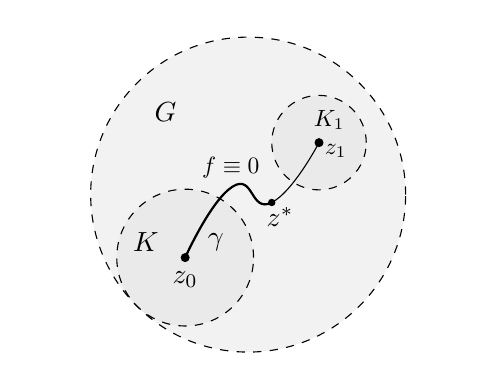
\begin{tikzpicture}
				\clip (-2.8, -2.14) rectangle (2.8, 2.12);
				
				\fill [opacity=0.05] (0,0) circle [radius=2];
				\draw[black, dashed] (0,0) circle[radius=2];
				
				\node[] at (-1.05, 1.05) {$G$};
				
				\fill [opacity=0.03] (0,0) (-0.8, -0.8) circle[radius=2 - 0.8 * 1.414];
				\draw[black,dashed] (-0.8, -0.8) circle[radius=2 - 0.8 * 1.41421];
				\node[] at (-1.3, -0.6) {$K$};
				\node[draw, circle, inner sep=1pt, fill, black, label=below:$z_0$] at (-0.8, -0.8) {};
				
				\node[] at (-0.41, -0.6) {$\gamma$};
				
				\fill [opacity=0.03] (0,0) (0.9, 0.66) circle[radius=0.6];
				\draw[black,dashed] (0.9, 0.66) circle[radius=0.6];
				\node[] at (1.03, 0.95) {\scalebox{0.85}{$K_1$}};
				\node[draw, circle, inner sep=1pt, fill, black, label={right, shift={(-3pt,-3pt)}:\scalebox{0.85}{$z_1$}}] at (0.9, 0.66) {};
				
				\path
				coordinate (start) at (-0.8, -0.8)
				coordinate (endd) at (0.9, 0.66);
				
				\begin{scope}
					\clip(-3, -2.5) rectangle (0.3, 1);
					\draw[style={thick}] plot [smooth, tension=0.9] coordinates {(start) (-0.2, 0.1) (0.3, -0.1) (endd)};
				\end{scope}
				
				\draw[] plot [smooth, tension=0.9] coordinates {(start) (-0.2, 0.1) (0.3, -0.1) (endd)};
				\node[draw, circle, inner sep=0.8pt, fill, black, label={below, shift={(3pt,3pt)}:$z^*$}] at (0.3, -0.1) {};
				\node[] at (-0.22, 0.34) {\scalebox{0.85}{$f \equiv 0$}};
			\end{tikzpicture}
		}
	\end{center}
	
	По предположению, $\tau \in (a, b)$ и, в силу непрерывности, $f(z^*) = 0$, причем нуль $z^*$ не является изолированным. Но тогда $f \equiv 0$ на некотором круге $K^*$ с центром в точке $z^*$, что противоречит выбору $\tau$.
\end{proof}

\begin{corollary}
	Пусть выполнены следующие условия:
	\begin{enumerate}
		\item Функции $g, h$ регулярны на области $G \subset \Cm$
		\item Множество $E \subset G$ "--- такое, что $g \equiv h$ на $E$
		\item $E$ имеет предельную точку $z_0 \in G$
	\end{enumerate}
	
	Тогда $g \equiv h$ на $G$.
\end{corollary}

\begin{proof}
	Применим теорему единственности к функции $g - h$, регулярной на области $G$.
\end{proof}

\begin{note}
	Из теоремы единственности также следует, что тот способ, которым мы доопределили экспоненту на $\Cm$, "--- единственный, при котором полученное продолжение является регулярным.
\end{note}

\begin{example}
	Рассмотрим следующее дифференциальное уравнение:
	\[y^{(n)} + a_1y^{(n-1)} + \dotsb + a_ny = 0\]
	
	Пусть $\widetilde y$ "--- некоторое частное решение уравнения. Тогда из теории дифференциальных уравнений мы знаем, какой вид имеет $\widetilde y$, и можем утверждать, что ее продолжение на $\Cm$ регулярно. Применяя теорему единственности к функции $g := \widetilde y^{(n)} + a_1\widetilde y^{(n-1)} + \dotsb + a_n\widetilde y$, получим, что $g \equiv 0$ не только на $\R$, но и на $\Cm$.
\end{example}